\documentclass[]{article}
\usepackage{mathtools}
\usepackage{graphicx}
\usepackage{hyperref}

%opening
\title{Visualizing Graduate Admissions Data \\ CMPS 161: Final Project}
\author{Aaron Doubek-Kraft \\ adoubekk@ucsc.edu}
\date{March 20, 2017}



\begin{document}
	
\begin{titlepage}

	\maketitle

	\begin{abstract}
		Abstract goes here!
	\end{abstract}

\end{titlepage}

\section{Introduction}
	In 2017, there were nearly 1100 applicants to the UC Santa Cruz graduate admissions program. Given the unusually large size of this applicant pool, making sense of any large-scale trends simply by looking at their records becomes an intractable problem. In addition to the high volume of applicants, the students' records contain a number of potentially interesting variables to be analyzed: quantitative data, including test scores and GPA, and qualitative data, such as the applicants' research interests, countries of origin, and other filters.  In this paper, I attempt to develop visualizations to identify correlations in this data that could be relevant to the selection process. I have attempted to make this paper accessible to a reader with no background in visualization by providing both high-level alongside technical descriptions of the problem and my approach.

\section{Approach}
	The large number of variables and the high volume of records to be analyzed makes this a classic multivariate visualization problem, and so I take a relatively standard approach: the parallel coordinate plot. In a typical graph, the number of variables available to be displayed is limited to 2 or 3, the number of spatial dimensions, so only correlations between 2 or 3 variables may be analyzed at a time (for example, in a scatter plot). The parallel coordinate plot generalizes this graphical approach 

	\begin{figure}[h]
		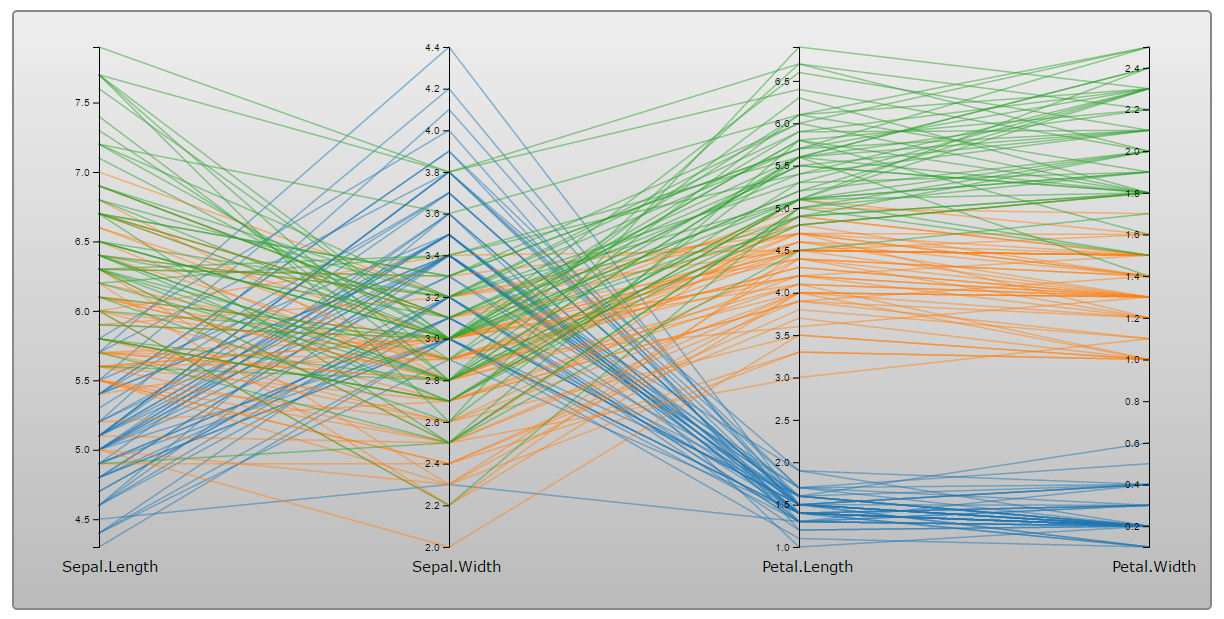
\includegraphics[width=\linewidth]{iris.png}
		\caption{Visualizing Edgar Anderson's Iris dataset. In this example, color is mapped to species of iris.}
		\label{fig:Result}
	\end{figure}	
\section{Implementation}
	\subsection{Processing Dataset}
	
\section{Results}

\section{Conclusion}

\begin{thebibliography}{11}
	\bibitem{datasets}
		R Datasets [Internet]. Available from: \url{https://vincentarelbundock.github.io/Rdatasets/datasets.html}
	\bibitem{telea}
		Telea, Alexandru C. Data Visualization Principles and Practice. 2nd Edition. Boca Raton(FL): CRC Press; 2015.
	\bibitem{kosara}
		Kosara, Robert. Parallel Coordinates [Internet]. Eagereyes; 2010. Available from \url{https://eagereyes.org/techniques/parallel-coordinates}
	\bibitem{bostock}
		Bostock, Mike. Parallel Coordinates Example [Internet]. d3.js; Available from \url{http://mbostock.github.io/d3/talk/20111116/iris-parallel.html}
\end{thebibliography}


\end{document}